\chapter{Istniejące rozwiązania}

W tym rozdziale przedstawię istniejące aplikacje internetowe \cite{mathex} i desktopowe służące do tworzenia i wizualizacji grafów. Tabela \ref{tab:app-comparison} zawiera porównanie funkcjonalności opisywanych darmowych aplikacji internetowych. 

Głównie skupię się na aplikacjach internetowych ze względu na związek z tematem mojej pracy. 

\section{Aplikacje internetowe}

\subsection*{Graph Creator}
\bigskip
\noindent\begin{tabularx}{\textwidth}{r|X|}
\cline{2-2}
  Adres URL & http://illuminations.nctm.org/Activity.aspx?id=3550 \\ 
\cline{2-2}
 Autor & National Council of Teachers of Mathematics \\ 
\cline{2-2}
 Licencja & Darmowa\\  
\cline{2-2}
\end{tabularx} 
\bigskip

Aplikacja pozwala tworzyć grafy skierowane i nieskierowane. Posiada możliwość kolorowania wierzchołków, wyrównania ich do siatki oraz ustawienia wag na krawędziach i etykiet w wierzchołkach. Ponadto użytkownik może wyświetlić stopnie wierzchołków oraz wyginać krawędzie. Dodatkową funkcjonalnością jest możliwość zaznaczenia kilku wierzchołków na raz. 

\textit{Graph Creator} nie daje możliwości eksportowania i importowania grafów. Nie można również przesuwać widoku ani oddalać oraz przybliżać grafu. Aplikacja posiada ograniczenie liczby wierzchołków -- maksymalna dozwolona ilość to 52 wierzchołki.

\begin{figure}[H]
\caption{Zrzut ekranu z aplikacji Graph Creator}
\centering
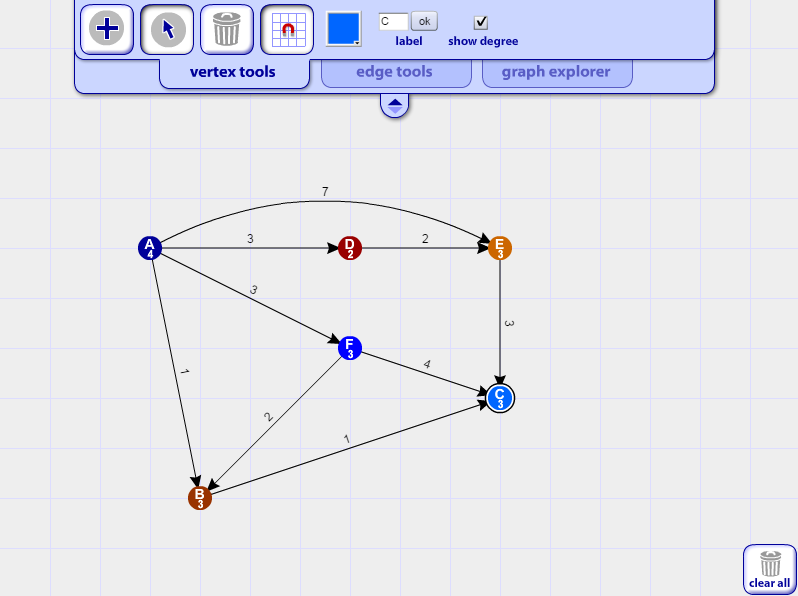
\includegraphics[width=\textwidth]{graph-creator.png}
\end{figure}

\subsection*{Graph Online}
\bigskip
\noindent\begin{tabularx}{\textwidth}{r|X|}
\cline{2-2}
  Adres URL & http://graphonline.ru/en/ \\ 
\cline{2-2}
 Autor & Unick-soft \\ 
\cline{2-2}
 Licencja & Darmowa\\  
\cline{2-2}
\end{tabularx} 
\bigskip

Aplikacja również daje możliwość stworzenia grafów zarówno skierowanych jak i nieskierowanych. Podobnie jak poprzednia aplikacja pozwala na zmianę etykiet wierzchołków, nadanie wag krawędziom oraz na wyświetlenie stopnia wierzchołków. Ponadto użytkownik ma możliwość przesuwania widoku oraz jego przybliżania i oddalania. Dodatkowo \textit{Graph Online} pozwala zapisać graf jako macierz sąsiedztwa lub incydencji oraz wczytać graf zapisany w takiej postaci. Użytkownik może również zapisać graf na serwerze -- po zapisaniu wyświetlany jest ogólnodostępny adres URL do grafu. Ciekawą funkcjonalnością jest eksport grafu do obrazka (plik \texttt{PNG}).

\textit{Graph Online} posiada możliwość wykonania podstawowych algorytmów na grafie, takich jak: znajdowanie najkrótszej ścieżki pomiędzy dwoma wierzchołkami, znajdowanie cyklu Eulera, znajdowanie spójnych składowych, znajdowanie minimalnego drzewa rozpinającego.  

W przeciwieństwie do poprzedniej aplikacji nie mamy możliwości kolorowania wierzchołków, zaznaczania kilku wierzchołków na raz oraz wyginania krawędzi. Maksymalna dozwolona ilość wierzchołków to 299. 

\begin{figure}[H]
\caption{Zrzut ekranu z aplikacji Graph Online}
\centering
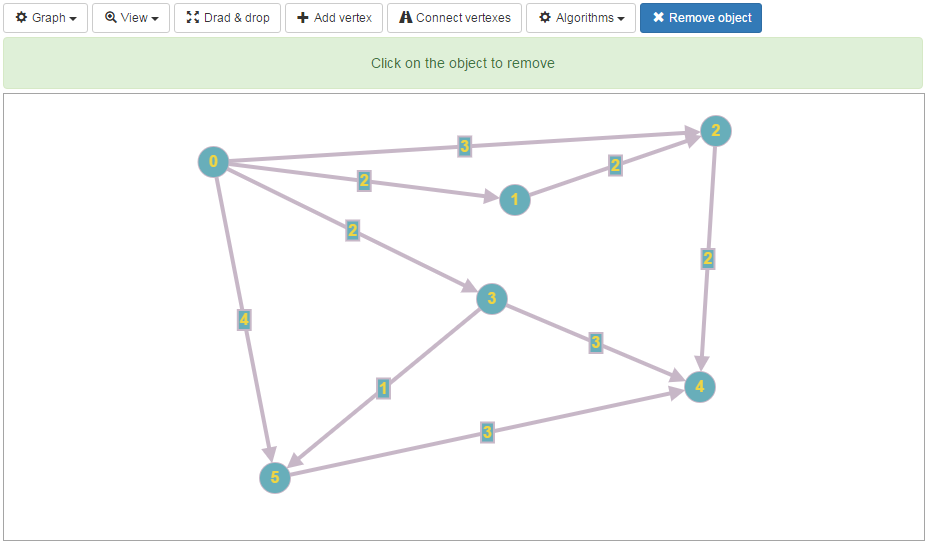
\includegraphics[width=\textwidth]{graph-online.png}
\end{figure}

\subsection*{GraphJS}
\bigskip
\noindent\begin{tabularx}{\textwidth}{r|X|}
\cline{2-2}
  Adres URL & https://dl.dropboxusercontent.com/u/4189520/GraphJS/ graphjs.html \\ 
\cline{2-2} 
 Autor & David Kofoed Wind \\ 
\cline{2-2}
 Licencja & Darmowa\\  
\cline{2-2}
\end{tabularx}
\bigskip

Aplikacja pozwala na tworzenie grafów nieskierowanych. Podobnie jak w poprzednich aplikacjach możemy nadawać etykiety wierzchołkom i krawędziom. Niespotykaną funkcjonalnością jest możliwość stworzenia kilku grafów i przełączania się pomiędzy nimi oraz możliwość eksportu grafu do formatu \LaTeX (pakiet Ti\textit{k}Z). Ponadto użytkownik ma możliwość eksportu do własnego formatu \texttt{JSON} oraz importu grafu z tego formatu. Aplikacja posiada funkcjonalność zaznaczania wielu wierzchołków na raz.

W \textit{GraphJS} nie ma możliwości przesuwania widoku oraz przybliżania i~oddalania grafu. Nie ma również możliwości kolorowania wierzchołków oraz wyginania krawędzi. Aplikacja zdaje się nie mieć limitu na liczbę wierzchołków -- udało się wczytać graf $C_{1000}$ jednakże dodanie kolejnego wierzchołka zajmuje około 10 sekund.

\begin{figure}[H]
\caption{Zrzut ekranu z aplikacji GraphJS}
\centering
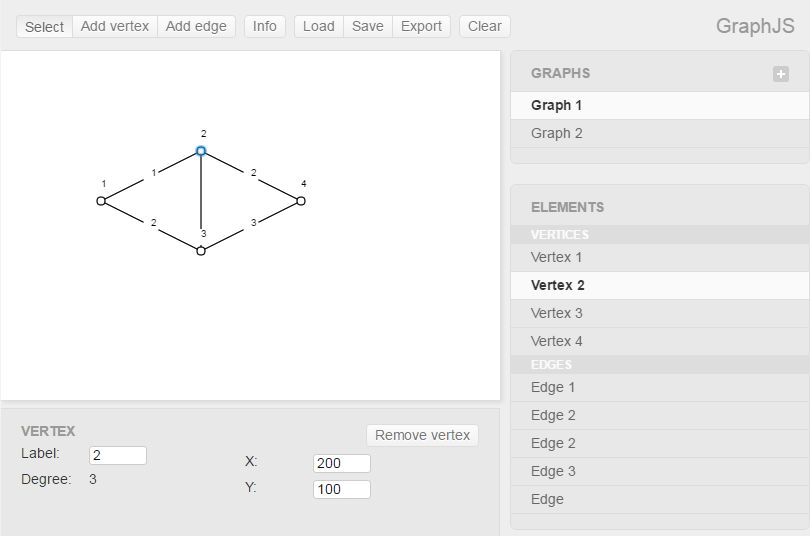
\includegraphics[width=\textwidth]{graphjs.png}
\end{figure}


\subsection*{Graphrel}
\bigskip
\noindent\begin{tabularx}{\textwidth}{r|X|}
\cline{2-2}
  Adres URL & https://yiboyang.github.io/graphrel/ \\ 
\cline{2-2} 
 Autor & Yibo Yang \\
\cline{2-2}
 Licencja & Darmowa\\  
\cline{2-2}
\end{tabularx} 
\bigskip

Aplikacja daje możliwość tworzenia grafów skierowanych. W przeciwieństwie do poprzednio opisywanych aplikacji posiada układ kierowany siłą (ang. \textit{force-directed layout}), choć istnieje również opcja samodzielnego rozstawienia wierzchołków -- poprzez przytrzymanie klawisza \texttt{Ctrl}. Użytkownik może zaimportować graf z formatu stworzonego przez aplikację (tablice list sąsiedztwa dla każdego wierzchołka). Bardzo przydatną i niespotykaną funkcjonalnością jest możliwość cofania oraz ponawiania ostatnich akcji. 

W \textit{Graphrel} nie możemy nadawać własnych etykiet na krawędziach ani w wierzchołkach, nie możemy przesuwać widoku ani zmieniać przybliżenia grafu. Nie ma również możliwości wyginania krawędzi, zaznaczania kliku wierzchołków na raz oraz kolorowania wierzchołków. Do aplikacji udało się wczytać graf $C_{100}$, przy próbie wczytania $C_{101}$ pojawia się informacja o niepoprawnym formacie.

\begin{figure}[H]
\caption{Zrzut ekranu z aplikacji Graphrel}
\centering
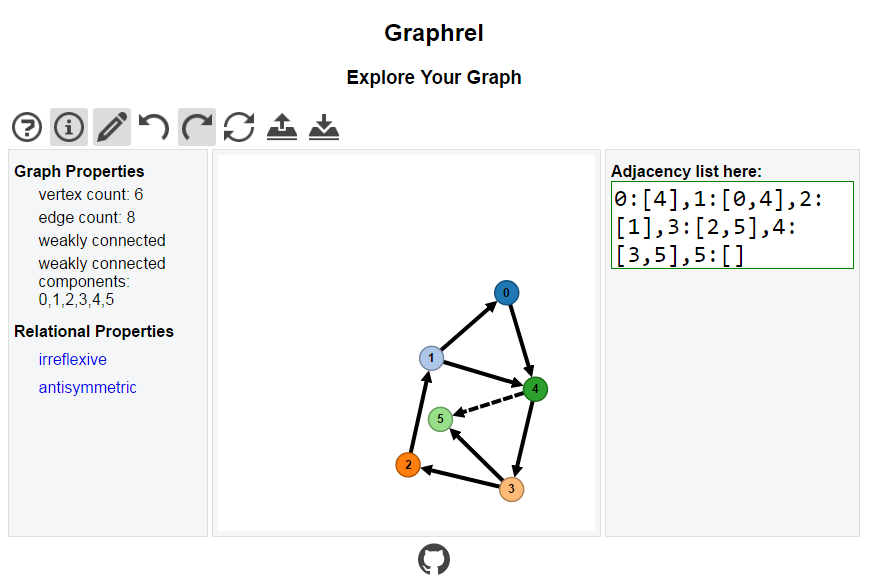
\includegraphics[width=\textwidth]{graphrel.png}
\end{figure}

\subsection*{VisuAlgo}
\bigskip
\noindent\begin{tabularx}{\textwidth}{r|X|}
\cline{2-2}
  Adres URL & https://visualgo.net/en/ \\ 
\cline{2-2} 
 Autor & Dr Steven Halim \\ 
\cline{2-2}
 Licencja & Darmowa\\ 
\cline{2-2}
\end{tabularx} 
\bigskip

Aplikacja stworzona przez Dr Stevena Halima z National University of Singapore. Posiada możliwość tworzenia prostych grafów, jednak jej głównym celem nie jest tworzenie grafów, lecz wizualizacja algorytmów przez animację (nie tylko na grafach, ale również na strukturach danych). Użytkownik wraz z przebiegiem algorytmu może obserwować przebieg kodu, może zatrzymać się w dowolnym jego kroku, cofnąć się do kroku poprzedniego albo przejść do następnego.

\begin{figure}[H]
\caption{Zrzut ekranu z aplikacji VisuAlgo}
\centering
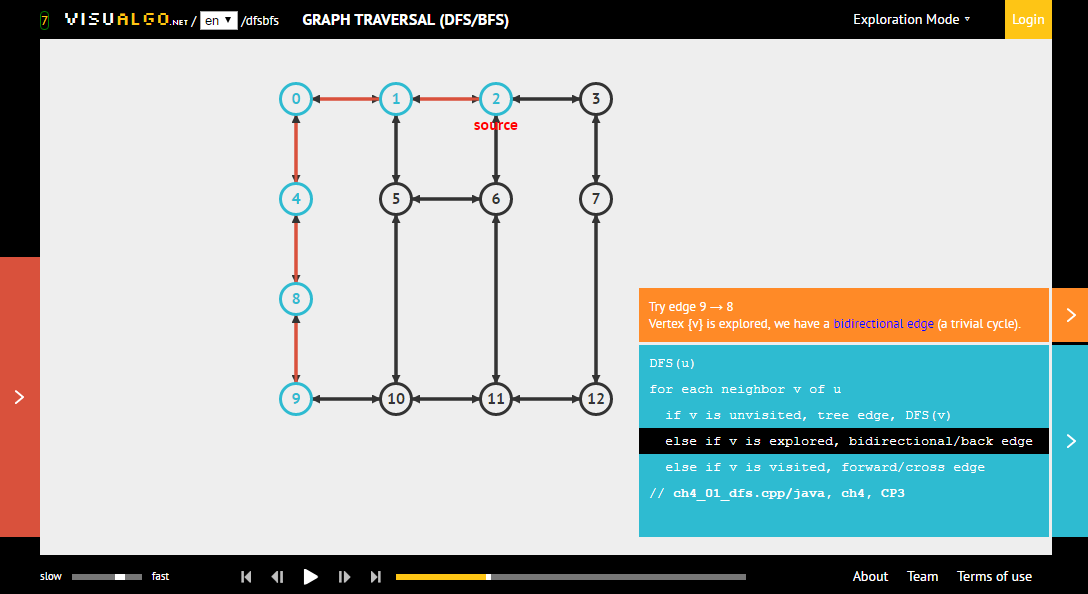
\includegraphics[width=\textwidth]{visualgo.png}
\end{figure}

\subsection*{yEd Live}
\bigskip
\noindent\begin{tabularx}{\textwidth}{r|X|}
\cline{2-2}
  Adres URL & https://www.yworks.com/yed-live/ \\ 
\cline{2-2} 
 Autor & yWorks\\ 
\cline{2-2}
 Licencja & Darmowa i płatna\\ 
\cline{2-2}
\end{tabularx}
\bigskip

Internetowa wersja aplikacji yEd stworzona przez firmę yWorks. Pozwala na tworzenie dowolnych grafów (skierowanych, nieskierowanych). W aplikacji istnieje możliwość nadawania etykiet wierzchołkom i krawędziom. Twórcy dostarczyli również możliwość kolorowania wierzchołków, zmiany ich kształtu, a nawet ustawiania obrazków w wierzchołkach. Użytkownik może też dowolnie wyginać krawędzie. Niespotykaną funkcjonalnością jest możliwość grupowania wierzchołków. 

Jeśli chodzi o wyświetlanie grafu, to \textit{yEd Live} dostarcza mały podgląd grafu, dzięki któremu możemy przesuwać graf. Istnieje też opcja przybliżania i oddalania grafu. Dodatkową funkcjonalnością jest zmiana układu wierzchołków (m.in. na układ hierarchiczny, ortogonalny czy kołowy) oraz wyszukiwanie wierzchołków po etykiecie.

W \textit{yEd Live} możemy zaimportować graf w formacie \texttt{GraphML} (z chmury, dysku lub adresu \texttt{URL}). Istnieje również możliwość eksportu do tegoż formatu oraz do pliku graficznego w formacie \texttt{PNG}. 

Aplikacja dostępna jest w dwóch wersjach: darmowej i płatnej. Darmowa wersja posiada pewne ograniczenia, np. możemy zapisać do formatu \texttt{GraphML} graf mający maksymalnie 25 wierzchołków oraz wyeksportować graf do pliku \texttt{PNG} mający maksymalnie 50 wierzchołków. 

\begin{figure}[H]
\caption{Zrzut ekranu z aplikacji yEd Live}
\centering
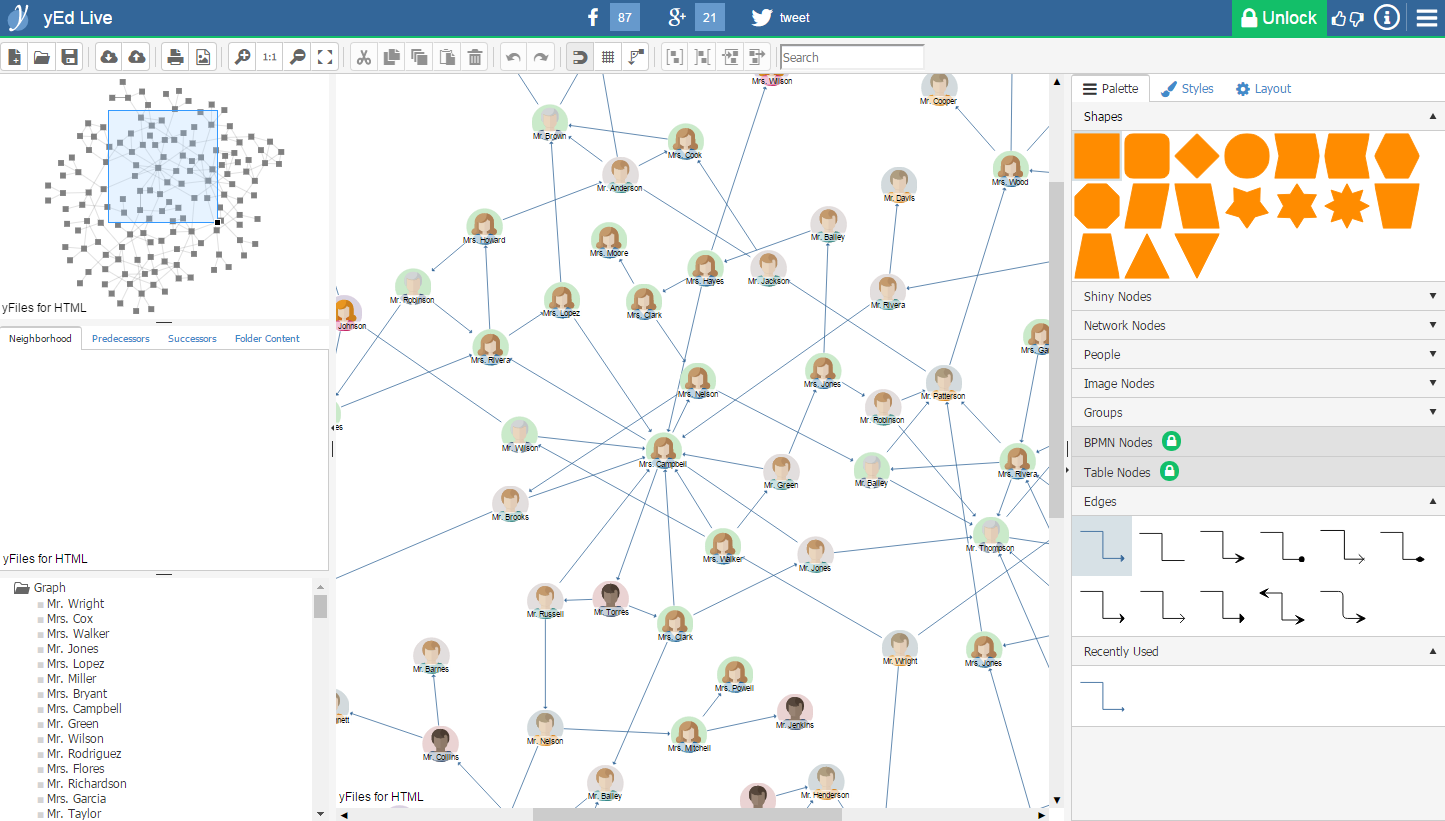
\includegraphics[width=\textwidth]{yed-live.png}
\end{figure}


\subsection*{Linkurious}
\bigskip
\noindent\begin{tabularx}{\textwidth}{r|X|}
\cline{2-2}
  Adres URL & http://linkurio.us \\ 
\cline{2-2} 
 Autor & Linkurious\\ 
\cline{2-2}
 Licencja & Płatna\\ 
\cline{2-2}
\end{tabularx}
\bigskip

Komercyjna aplikacja internetowa służąca do wizualizacji i badania grafowych baz danych\footnote{Wspierane bazy danych: \textit{Neo4j}, \textit{DataStax Enterprise Graph}, \textit{Titan}, \textit{AllegroGraph} oraz ich języki zapytań: \textit{Cypher}, \textit{Gremlin} i \textit{SPARQL}.}. Jej współzałożycielem jest Dr Sébastien Heymann -- współtwórca aplikacji desktopowej Gephi służącej również do wizualizacji i analizowania grafów. 

Aplikacja wspiera duże zbiory danych -- grafy z miliardami wierzchołków i krawędzi \cite{linkurious}. Pozwala na współpracę wielu użytkowników, m.in. przez możliwość udostępniania grafów czy publikowanie wizualizacji w czasie rzeczywistym. 

Posiada kilka opcji układów grafów (kierowanych siłą i hierarchicznych). Dostarcza również możliwość widoku geoprzestrzennego. 

W \textit{Linkurious} istnieje możliwość dostosowania wyglądu elementów, np. wielkość wierzchołków, grubość krawędzi, zmiana ikon w wierzchołkach, tak aby wizualizacje były bogate w informacje. Użytkownik może również tworzyć filtry, by wyświetlić tylko istotne dane oraz tworzyć powiadomienia o podejrzanych połączeniach. 

\begin{figure}[H]
\caption{Zrzut ekranu z aplikacji Linkurious}
\centering
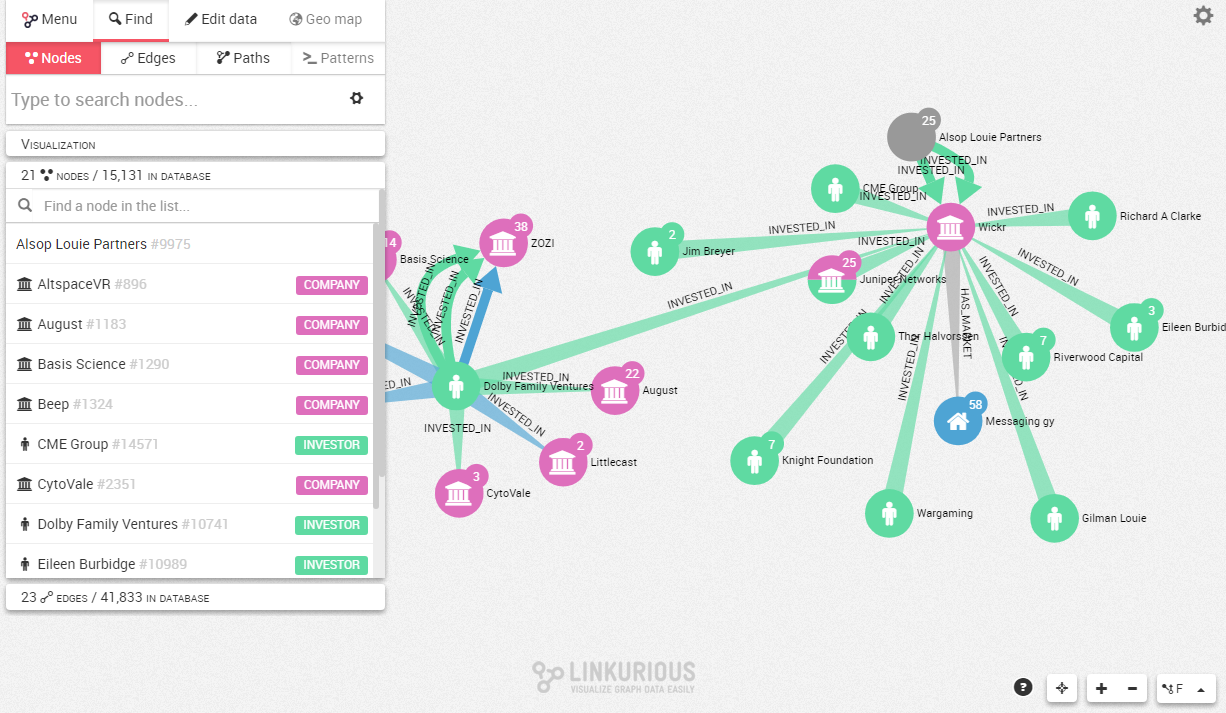
\includegraphics[width=\textwidth]{linkurious.png}
\end{figure}

\begin{table}[H]
\centering
\begin{threeparttable}
\caption{Porównanie darmowych aplikacji \textit{Graph Creator}, \textit{Graph Online}, \textit{GraphJS}, \textit{Graphrel} i \textit{yEd Live}}
\label{tab:app-comparison}
\begin{tabular}{ r|c|c|c|c|c| } 
\multicolumn{1}{r}{}
 &  \multicolumn{1}{c}{\rotatebox{70}{Graph Creator}}
 & \multicolumn{1}{c}{\rotatebox{70}{Graph Online}} 
 & \multicolumn{1}{c}{\rotatebox{70}{GraphJS}} 
 & \multicolumn{1}{c}{\rotatebox{70}{Graphrel}} 
 & \multicolumn{1}{c}{\rotatebox{70}{yEd Live}} \\
\cline{2-6}
graf nieskierowany & \checkmark & \checkmark  & \checkmark  & -- & \checkmark \\
\cline{2-6}
graf skierowany  & \checkmark & \checkmark  & --  & \checkmark & \checkmark \\
\cline{2-6}
etykiety na krawędziach  & \checkmark & \checkmark  & \checkmark  & -- & \checkmark \\
\cline{2-6}
etykiety w wierzchołkach & \checkmark & \checkmark  & \checkmark  & -- & \checkmark \\
\cline{2-6}
kolorowanie wierzchołków & \checkmark & --  & --  & -- & \checkmark \\
\cline{2-6}
łuki jako krawędzie & \checkmark & --  & --  & -- & \checkmark \\
\cline{2-6}
zaznaczanie kilku wierzchołków & \checkmark & --  & \checkmark  & -- & \checkmark \\
\cline{2-6}
grupowanie wierzchołków & -- & --  & --  & -- & \checkmark \\
\cline{2-6}
przesuwanie widoku & -- & \checkmark  & --  & -- & \checkmark \\
\cline{2-6}
przybliżanie/oddalanie & -- & \checkmark  & --  & -- & \checkmark \\
\cline{2-6}
zapisywanie/wczytywanie & -- & \checkmark\tnote{1}  & \checkmark\tnote{2}  & \checkmark\tnote{3} & \checkmark\tnote{4} \\
\cline{2-6}
\end{tabular}
\begin{tablenotes}
{\footnotesize\bigskip
\item[1] jako macierz sąsiedztwa lub jako obrazek
\item[2] własny format \texttt{JSON} lub jako \LaTeX
\item[3] własny format (listy sąsiedztwa)
\item[4] \texttt{GraphML} lub jako obrazek (w wersji darmowej jest ograniczenie na
 wielkość zapisywanego grafu)
}
\end{tablenotes}
\end{threeparttable}
\end{table}

\section{Aplikacje desktopowe}

Istnieje również szereg aplikacji desktopowych służących do wizualizacji, analizy i edycji grafów. Są one bardziej rozbudowane i zakres ich funkcjonalności jest znacznie szerszy od aplikacji internetowych. Do najbardziej znanych należą \cite{mathex-desktop}:

\begin{itemize}
\setlength\itemsep{0em}
\item \href{https://gephi.org/}{Gephi}
\item \href{http://www.graphtheorysoftware.com/}{GraphTea}
\item \href{http://www.cytoscape.org/}{Cytoscape}
\item \href{https://www.yworks.com}{yEd Graph Editor}
\end{itemize}

\begin{figure}[H]
\caption{Zrzut ekranu z aplikacji Gephi}
\centering
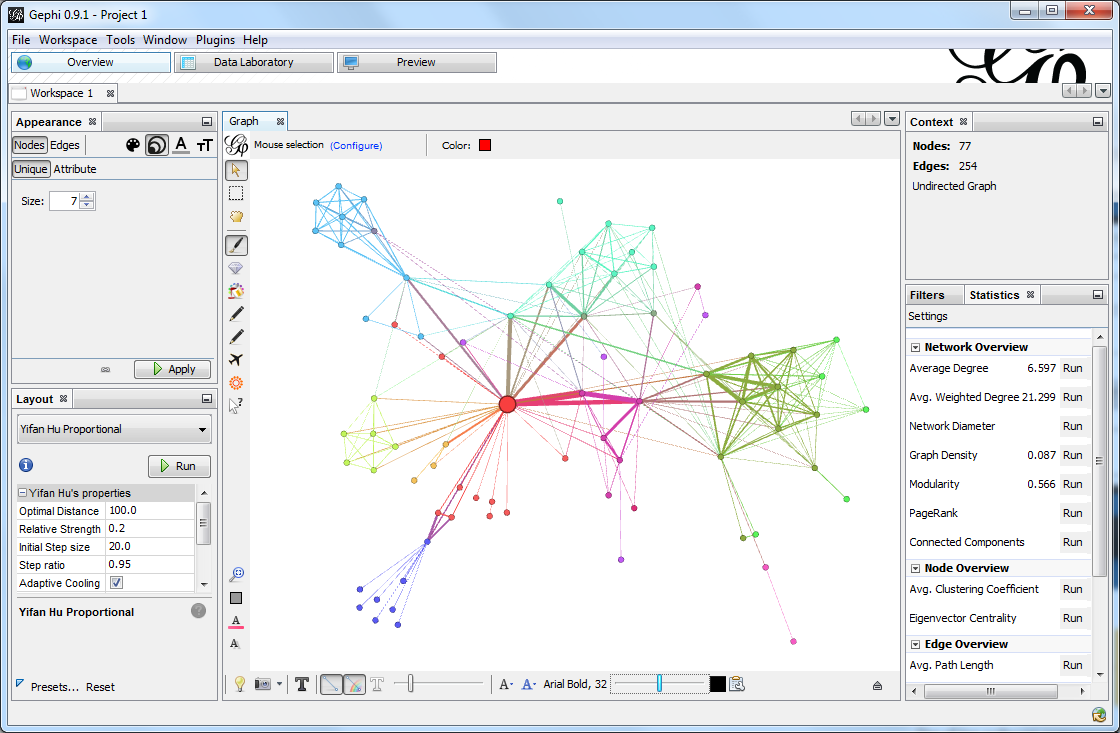
\includegraphics[width=\textwidth]{gephi.png}
\end{figure}
